\documentclass[aspectratio=169,10pt]{beamer}

% =================================================
% 1. THEME AND FONTS
% =================================================

\usetheme{Madrid}
\useoutertheme{infolines}
\usefonttheme{professionalfonts}

\usepackage{iftex}

\ifXeTeX
    \usepackage{fontspec}
    \setmainfont{Carlito}
\else
    \usepackage[T1]{fontenc}
    \usepackage[sfdefault]{carlito}
\fi

% =================================================
% 2. PACKAGES
% =================================================

\usepackage{graphicx}
\usepackage{booktabs}
\usepackage{tabularx}
\usepackage{array}
\usepackage{tikz}
\usepackage{ragged2e}
\usepackage{amsmath}

\usetikzlibrary{positioning,arrows.meta}

% =================================================
% 3. STRATHMORE COLOUR SCHEME
% =================================================

\definecolor{StrathBlue}{HTML}{2A4591}
\definecolor{StrathRed}{HTML}{C8282A}
\definecolor{StrathGold}{HTML}{C5A044}
\definecolor{SoftBlue}{HTML}{F1F4FA}
\definecolor{Muted}{HTML}{687386}

\setbeamercolor{structure}{fg=StrathBlue}

\setbeamercolor{palette primary}{
    bg=StrathBlue,
    fg=white
}

\setbeamercolor{palette secondary}{
    bg=StrathBlue!88!black,
    fg=white
}

\setbeamercolor{palette tertiary}{
    bg=StrathBlue!75!black,
    fg=white
}

\setbeamercolor{palette quaternary}{
    bg=StrathRed,
    fg=white
}

\setbeamercolor{frametitle}{
    bg=StrathBlue,
    fg=white
}

\setbeamercolor{block title}{
    bg=StrathBlue,
    fg=white
}

\setbeamercolor{block body}{
    bg=SoftBlue,
    fg=black
}

\setbeamercolor{alerted text}{
    fg=StrathRed
}

% =================================================
% 4. PRESENTATION FORMATTING
% =================================================

\setbeamertemplate{navigation symbols}{}

\setbeamertemplate{itemize item}{
    \color{StrathGold}\small$\blacktriangleright$
}

\setbeamertemplate{frametitle}{
    \nointerlineskip
    \begin{beamercolorbox}[
        wd=\paperwidth,
        ht=.76cm,
        dp=.2cm,
        leftskip=.35cm
    ]{frametitle}
        \usebeamerfont{frametitle}
        \insertframetitle
    \end{beamercolorbox}

    
\begin{tikzpicture}
        \draw[
            StrathGold,
            line width=1.1pt
        ] (0,0)--(\paperwidth,0);
    \end{tikzpicture}
}

% =================================================
% 5. IMAGE PATHS
% =================================================

% Relative paths: work when compiled from reports/final_report
% (or from the repository root), on any computer.
\graphicspath{{../figures/}{reports/figures/}{./}{reports/final_report/}}

\newcommand{\StrathLogo}{Strathmore logo.png}

% =================================================
% 6. FOOTER
% =================================================

\setbeamertemplate{footline}{
    \leavevmode
    \hbox{
        \begin{beamercolorbox}[
            wd=.30\paperwidth,
            ht=2.6ex,
            dp=1ex,
            leftskip=1em
        ]{author in head/foot}
            \color{white}
            \scriptsize Faith Makena Riungu
        \end{beamercolorbox}

        \begin{beamercolorbox}[
            wd=.48\paperwidth,
            ht=2.6ex,
            dp=1ex,
            center
        ]{title in head/foot}
            \color{white}
            \scriptsize DSA 8401 | Applied Machine Learning
        \end{beamercolorbox}

        \begin{beamercolorbox}[
            wd=.22\paperwidth,
            ht=2.6ex,
            dp=1ex,
            center
        ]{date in head/foot}
            \color{white}
            \scriptsize
            \insertframenumber/\inserttotalframenumber
        \end{beamercolorbox}
    }
}

\setbeamercolor{author in head/foot}{
    bg=StrathBlue!90!black,
    fg=white
}

\setbeamercolor{title in head/foot}{
    bg=StrathBlue,
    fg=white
}

\setbeamercolor{date in head/foot}{
    bg=StrathRed,
    fg=white
}

% =================================================
% 7. TITLE INFORMATION
% =================================================

\title[Traditional Bank Use in Kenya]{
    Predicting Traditional Bank Use Among Kenyan Adults
}

\subtitle{
    A Machine Learning and Gender-Fairness Analysis
}

\author{
    Faith Makena Riungu
}

\institute{
    School of Computing and Engineering Sciences\\
    Strathmore University
}

\date{November 2026}

\titlegraphic{
    \includegraphics[height=1.2cm]{\StrathLogo}
}

% =================================================
% 8. DOCUMENT START
% =================================================

\begin{document}

% =================================================
% SLIDE 1: TITLE PAGE
% =================================================

{
\setbeamertemplate{footline}{}

\begin{frame}[plain]

\begin{tikzpicture}[remember picture,overlay]

    \fill[StrathBlue]
    (current page.north west)
    rectangle
    ([yshift=-.2cm]current page.north east);

    \fill[StrathGold]
    ([yshift=-.2cm]current page.north west)
    rectangle
    ([yshift=-.27cm]current page.north east);

\end{tikzpicture}

\titlepage

\begin{center}
    \small
    DSA 8401 | Applied Machine Learning Capstone Project
\end{center}

\end{frame}
}

% =================================================
% SLIDE 2: PRESENTATION OVERVIEW
% =================================================

\begin{frame}{Presentation overview}

\begin{columns}[T,onlytextwidth]

\column{.55\textwidth}

\begin{enumerate}
    \item Problem framing and objectives
    \item Data and target definition
    \item Modelling and validation
    \item Predictive performance
    \item Gender-fairness assessment
    \item Threshold mitigation
    \item Interpretation, deployment and limitations
\end{enumerate}

\column{.42\textwidth}

\begin{block}{Central question}

Can machine learning predict traditional bank use among Kenyan adults, and do its predictions perform differently for women and men?

\end{block}

\end{columns}

\end{frame}

% =================================================
% SLIDE 3: PROBLEM FRAMING
% =================================================

\begin{frame}{Problem framing and motivation}

\begin{block}{The problem}

Financial inclusion has expanded in Kenya, but access to financial services does not necessarily translate into use of traditional banking products.

\end{block}

\begin{itemize}

    \item Traditional bank use reflects demographic, socioeconomic and household circumstances.

    \item Machine learning can identify complex patterns across these characteristics.

    \item Strong aggregate performance may conceal unequal errors across population groups.

\end{itemize}

\begin{alertblock}{Research focus}

Evaluate predictive performance and examine whether model errors differ systematically by gender.

\end{alertblock}

\end{frame}

% =================================================
% SLIDE 4: OBJECTIVES AND QUESTIONS
% =================================================

\begin{frame}{Objective and research questions}

\textbf{Main objective}

Develop a machine learning model to predict traditional bank use among Kenyan adults and assess gender differences in its predictions.

\vspace{.2cm}

\begin{enumerate}

    \item How accurately can demographic, socioeconomic and household characteristics predict traditional bank use?

    \item Which candidate model performs best?

    \item Does model performance differ between women and men?

    \item Can threshold adjustment reduce observed disparities?

    \item Which features contribute most to predictions?

\end{enumerate}

\vspace{.15cm}

{\footnotesize\color{Muted}
The study is predictive and cross-sectional; it does not estimate causal effects.
}

\end{frame}

% =================================================
% SLIDE 5: DATA AND TARGET
% =================================================

\begin{frame}{Data and prediction target}

\begin{columns}[T,onlytextwidth]

\column{.48\textwidth}

\begin{block}{2024 FinAccess Household Survey}

\begin{itemize}

    \item Selected extract: 20,871 observations

    \item Adult analytical sample: 19,750

    \item Respondents aged 18 years and above

    \item Survey clusters and weights retained

\end{itemize}

\end{block}

\column{.48\textwidth}

\begin{block}{Binary classification}

\begin{itemize}

    \item Target: traditional bank use

    \item Usage = 1

    \item Non-usage = 0

    \item Gender reserved for fairness analysis, not used as a predictor

\end{itemize}

\end{block}

\end{columns}

\begin{alertblock}{Scope}

The target concerns traditional bank use, not overall financial inclusion or mobile-money access.

\end{alertblock}

\end{frame}

% =================================================
% SLIDE 6: ANALYTICAL WORKFLOW
% =================================================

\begin{frame}{Analytical workflow}

\centering

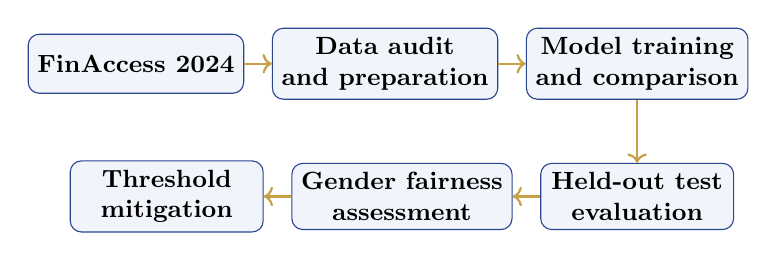
\begin{tikzpicture}[
    node distance=.35cm,
    boxstyle/.style={
        draw=StrathBlue,
        fill=SoftBlue,
        rounded corners,
        minimum width=2.45cm,
        minimum height=.75cm,
        align=center,
        font=\small\bfseries
    },
    arr/.style={
        ->,
        thick,
        draw=StrathGold
    }
]

\node[boxstyle] (a) {FinAccess 2024};

\node[boxstyle,right=of a] (b) {
    Data audit\\and preparation
};

\node[boxstyle,right=of b] (c) {
    Model training\\and comparison
};

\node[boxstyle,below=.8cm of c] (d) {
    Held-out test\\evaluation
};

\node[boxstyle,left=of d] (e) {
    Gender fairness\\assessment
};

\node[boxstyle,left=of e] (f) {
    Threshold\\mitigation
};

\draw[arr] (a)--(b);
\draw[arr] (b)--(c);
\draw[arr] (c)--(d);
\draw[arr] (d)--(e);
\draw[arr] (e)--(f);

\end{tikzpicture}

\vspace{.45cm}

\begin{itemize}

    \item Missing values, inconsistent responses and duplicates were audited.

    \item Preprocessing was fitted within training folds to reduce leakage.

    \item Model interpretation and a prediction API completed the workflow.

\end{itemize}

\end{frame}

% =================================================
% SLIDE 7: MODELS AND VALIDATION
% =================================================

\begin{frame}{Candidate models and validation strategy}

\begin{columns}[T,onlytextwidth]

\column{.46\textwidth}

\textbf{Models evaluated}

\begin{itemize}

    \item Dummy prior baseline

    \item Logistic Regression

    \item Random Forest

    \item Histogram-based Gradient Boosting

\end{itemize}

\vspace{.2cm}

\textbf{Selection metric}

Survey-weighted PR-AUC.

\column{.50\textwidth}

\textbf{Validation design}

\begin{itemize}

    \item Cluster-aware stratified group splitting.

    \item One group-held-out test set (3,942 respondents).

    \item Nested group-aware cross-validation.

    \item Survey weights used in fitting and evaluation.

    \item Test set excluded from model and threshold selection.

\end{itemize}

\end{columns}

\end{frame}

% =================================================
% SLIDE 8: CROSS-VALIDATION RESULTS
% =================================================

\begin{frame}{Model comparison: cross-validation}

\small

\begin{table}

\centering

\begin{tabular}{lcc}

\toprule

\textbf{Model}
&
\textbf{Weighted PR-AUC}
&
\textbf{Fold SD}
\\

\midrule

Gradient Boosting
&
\textbf{0.712}
&
0.029
\\

Random Forest
&
0.703
&
0.034
\\

Logistic Regression
&
0.694
&
0.035
\\

Dummy baseline
&
0.286
&
0.006
\\

\bottomrule

\end{tabular}

\end{table}

\begin{block}{Model selected}

Gradient Boosting achieved the highest mean survey-weighted PR-AUC and was selected as the champion model.

\end{block}

\begin{alertblock}{Interpretation}

Its lead over Random Forest was modest (about 0.009), smaller than fold-to-fold variability; this is not decisive superiority.

\end{alertblock}

\end{frame}

% =================================================
% SLIDE 9: TEST PERFORMANCE
% =================================================

\begin{frame}{Held-out test performance}

\begin{columns}[T,onlytextwidth]

\column{.48\textwidth}

\begin{block}{Weighted PR-AUC}

\centering

{\LARGE\bfseries\color{StrathBlue}0.753}

\end{block}

\begin{block}{Weighted ROC-AUC}

\centering

{\LARGE\bfseries\color{StrathBlue}0.871}

\end{block}

\begin{block}{Weighted F1 at 0.50}

\centering

{\LARGE\bfseries\color{StrathBlue}0.668}

\end{block}

\column{.48\textwidth}

\begin{itemize}

    \item Test sample: 3,942 respondents.

    \item Weighted outcome prevalence: 30.4\%.

    \item Weighted precision: 73.3\%.

    \item Weighted recall: 61.3\%.

    \item Weighted Brier score: 0.131.

\end{itemize}

\end{columns}

\vspace{.1cm}

{\footnotesize\color{Muted}
Classification metrics use the original 0.50 threshold unless otherwise stated.
}

\end{frame}

% =================================================
% SLIDE 10: GENDER FAIRNESS
% =================================================

\begin{frame}{Gender fairness: the recall gap}

\begin{columns}[T,onlytextwidth]

\column{.56\textwidth}

\begin{table}

\centering

\begin{tabular}{lcc}

\toprule

&
\textbf{Women}
&
\textbf{Men}
\\

\midrule

Weighted recall
&
\textbf{51.9\%}
&
\textbf{67.5\%}
\\

Weighted FPR
&
6.9\%
&
13.5\%
\\

Weighted PR-AUC
&
0.707
&
0.782
\\

\bottomrule

\end{tabular}

\end{table}

\column{.40\textwidth}

\begin{block}{Recall gap}

\centering

{\LARGE\color{StrathRed}\bfseries 15.6 pp}

\vspace{.1cm}

Male minus female recall

\end{block}

\end{columns}

\begin{alertblock}{95\% cluster-bootstrap CI}

7.2 to 23.1 percentage points.

\end{alertblock}

The model was less likely to correctly identify women who reported traditional bank use. Excluding gender from predictors did not remove the disparity.

\end{frame}

% =================================================
% SLIDE 11: THRESHOLD MITIGATION
% =================================================

\begin{frame}{Threshold mitigation: improvement with a trade-off}

\small

\begin{table}

\centering

\begin{tabular}{lccc}

\toprule

\textbf{Test measure}
&
\textbf{0.50}
&
\textbf{0.320}
&
\textbf{Change}
\\

\midrule

Weighted F1
&
0.668
&
0.690
&
+0.023
\\

Female recall
&
51.9\%
&
70.3\%
&
+18.4 pp
\\

Male recall
&
67.5\%
&
79.4\%
&
+11.9 pp
\\

Recall gap
&
15.6 pp
&
9.1 pp
&
-6.5 pp
\\

Weighted FPR
&
9.7\%
&
19.1\%
&
+9.4 pp
\\

\bottomrule

\end{tabular}

\end{table}

\begin{block}{What improved?}

A common threshold of 0.320, selected using training out-of-fold predictions, improved weighted F1 and narrowed the gender recall gap.

\end{block}

\begin{alertblock}{What is the trade-off?}

The gap remained and the false-positive rate increased substantially. Threshold adjustment is not a complete fairness solution.

\end{alertblock}

\end{frame}

% =================================================
% SLIDE 12: SHAP FEATURE IMPORTANCE
% =================================================

\begin{frame}{What informs the model's predictions?}

\begin{columns}[T,onlytextwidth]

\column{.56\textwidth}

\centering

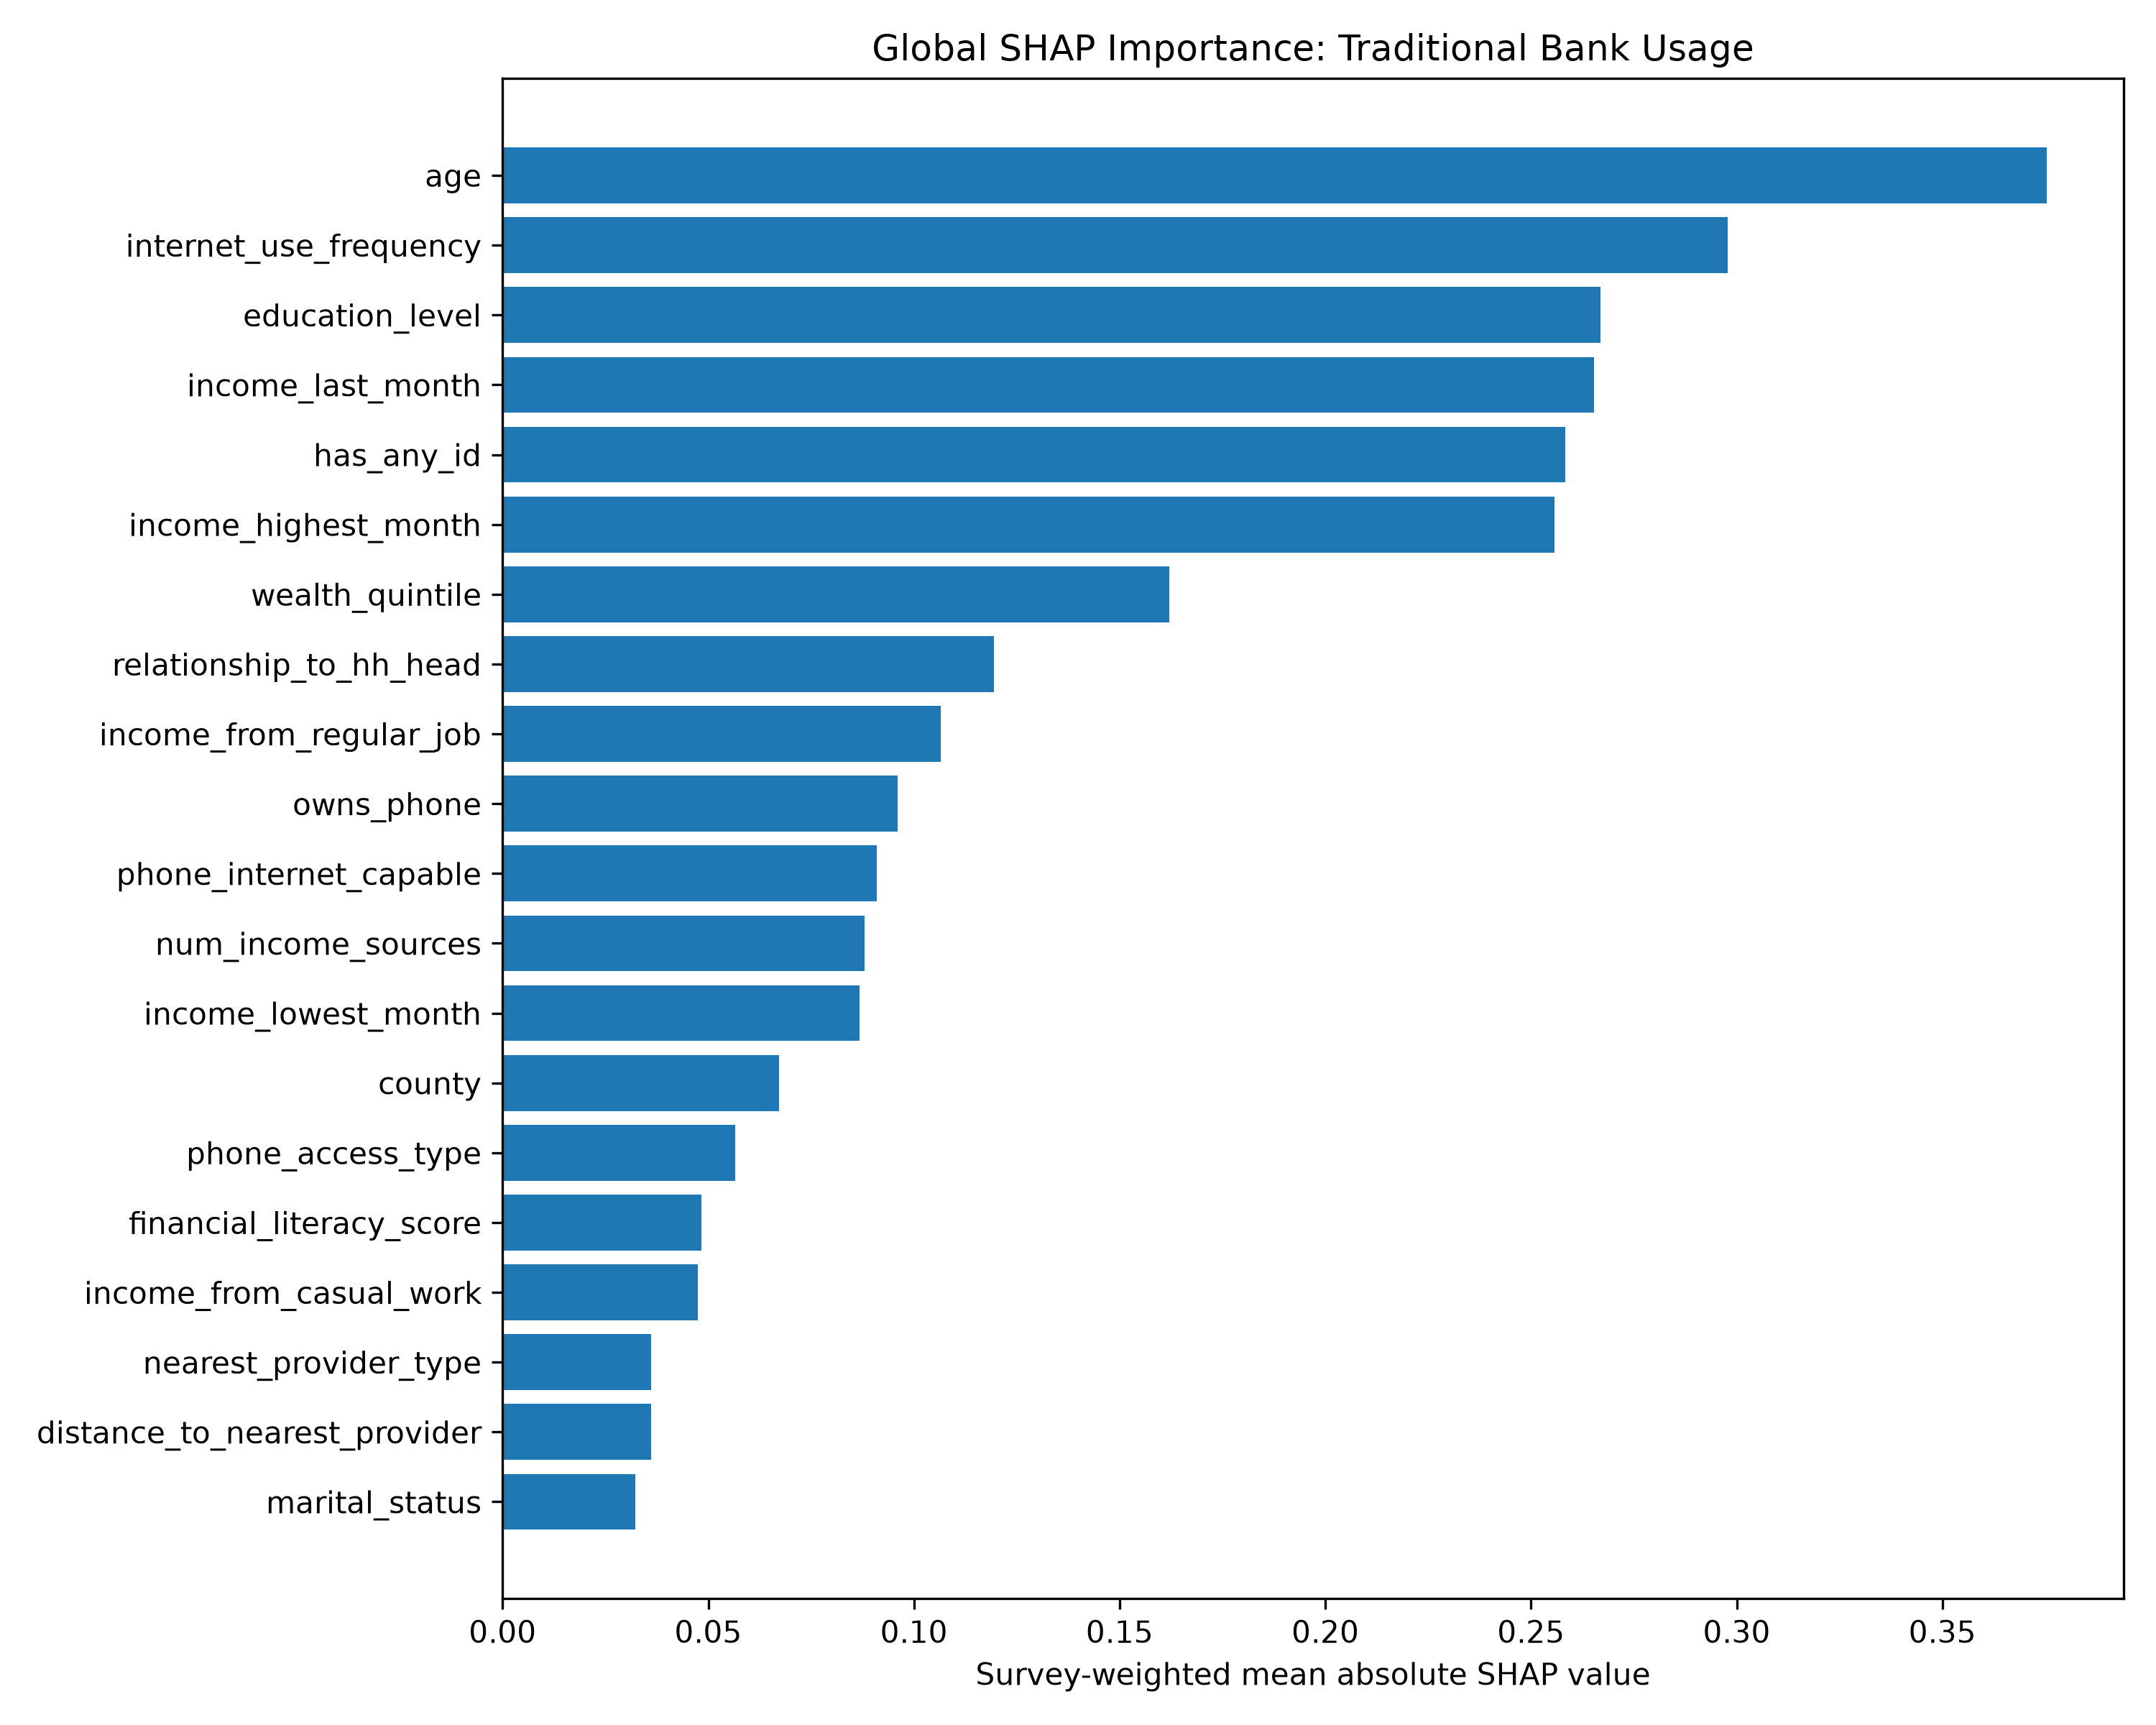
\includegraphics[
    width=\linewidth,
    height=5.0cm,
    keepaspectratio
]{shap_global_importance.png}

\column{.40\textwidth}

\textbf{Top predictors}
\begin{itemize}
    \item Age
    \item Internet-use frequency
    \item Education level
    \item Income (recent and highest month)
    \item Identity documentation
\end{itemize}

\vspace{.15cm}

\textbf{By gender}\\[2pt]
{\small Income and household position \emph{lower} women's scores but \emph{raise} men's, so more female bank users fall below the threshold.}

\vspace{.15cm}

{\footnotesize\color{Muted}
SHAP values describe model contribution, not causal effects.
}

\end{columns}

\end{frame}

% =================================================
% SLIDE 13: REPRODUCIBLE ARTEFACT
% =================================================

\begin{frame}{From analysis to a reproducible artefact}

\begin{columns}[T,onlytextwidth]

\column{.48\textwidth}

\begin{block}{Model package}

\begin{itemize}

    \item Fitted model and preprocessing

    \item Feature schema and metadata

    \item Common decision threshold

    \item Prediction and reason-code outputs

\end{itemize}

\end{block}

\column{.48\textwidth}

\begin{block}{Service layer}

\begin{itemize}

    \item FastAPI: predict, batch, health, metadata

    \item Invalid input rejected (HTTP 422)

    \item Docker: non-root, read-only, health check

    \item Container matches offline predictions

    \item 36 automated tests

\end{itemize}

\end{block}

\end{columns}

\begin{alertblock}{Deployment status}

A technical demonstration of a reproducible prediction workflow, not proof of production readiness for financial decisions.

\end{alertblock}

\end{frame}

% =================================================
% SLIDE 14: LIMITATIONS
% =================================================

\begin{frame}{Limitations and responsible interpretation}

\begin{itemize}

    \item \textbf{Cross-sectional data:}
    one survey round; later rounds and independent data are needed.

    \item \textbf{Prediction, not causation:}
    feature importance does not establish why people use banks.

    \item \textbf{Fairness is multidimensional:}
    reducing the recall gap increased false positives.

    \item \textbf{Gender can be inferred:}
    other predictors identify gender with AUC 0.91, so excluding it is not enough.

    \item \textbf{Subgroup variation:}
    recall at 0.50 is 49\% for rural women vs 74\% for urban men.

    \item \textbf{Responsible use:}
    predictions should not determine individual eligibility or exclusion.

\end{itemize}

\end{frame}

% =================================================
% SLIDE 15: CONCLUSION
% =================================================

\begin{frame}{Conclusion and recommendations}

\begin{block}{Conclusion}

Gradient Boosting provided useful predictive performance, but the fairness audit identified a material gender recall gap that excluding gender did not prevent. A common threshold of 0.320 narrowed the gap from 15.6 to 9.1 pp while doubling false positives.

\end{block}

\textbf{Recommendations}

\begin{enumerate}

    \item Report performance separately for women and men.

    \item Select thresholds transparently and evaluate multiple error measures.

    \item Validate on later FinAccess rounds and independent data.

    \item Investigate gender and geographic disparities beyond threshold adjustment.

    \item Treat the model as an analytical support tool, not an eligibility decision system.

\end{enumerate}

\end{frame}

% =================================================
% SLIDE 16: THANK YOU
% =================================================

{
\setbeamertemplate{footline}{}

\begin{frame}[plain]

\centering

\vspace{.8cm}

\includegraphics[
    height=1.3cm
]{\StrathLogo}

\vspace{.6cm}

{\Huge\bfseries\color{StrathBlue}Thank you}

\vspace{.25cm}

{\Large Questions}



\end{frame}
}

% =================================================
% END DOCUMENT
% =================================================

\end{document}